
\documentclass[11pt ,A4]{article}
% \usepackage{amsmath} % \usepackage is a command that allows you to add functionality to your LaTeX code
\usepackage[a4paper, total={7in, 9in}]{geometry}
% \usepackage[sfdefault]{roboto}

\usepackage[none]{hyphenat}
% \usepackage{url}
\usepackage[colorlinks=true, allcolors=blue]{hyperref}
\usepackage{indentfirst}

\usepackage{graphicx}
\graphicspath{ {./images/} }

\setlength{\parindent}{0.5cm}

\title{Jocului Vieții\\Proiectul 6}
\author{Capisizu Cosmin Louis\\IS1.1} % Sets authors name
% \date{\today}

\begin{document}
    \maketitle % creates title using information in preamble (title, author, date)
    \pagebreak

    \section{Cerința} % creates a section
        \paragraph{}
            Proiectarea si implementarea unui sistem multi-agent pentru simularea jocului vieții, game of life. Se va defini si analiza cel putin un joc de tip automat celular diferit de cel din programul demonstrativ pentru jocul vietii. Pentru jocul vietii se vor defini si experimenta si alte configuratii initiale, pe langa cele predefinite in programul demonstrativ.

    \section{Prezentarea jocului}

        \paragraph{}Jocul Vietii, cunoscut si sub numele de Viata, este un automat celular conceput de matematicianul britanic John Horton Conway in 1970. Este un joc fara jucatori, ceea ce inseamna ca evolutia sa este determinata de starea sa initiala, nefiind nevoie de alte informatii.

        \paragraph{} Se interactioneaza cu Jocul Vietii creand o configuratie initiala si observand cum evolueaza. Este Turing complet si poate simula un constructor universal sau orice alta masina Turing.

        \paragraph{} Universul Jocului Vietii este o retea ortogonala infinita, bidimensionala, de celule patrate, fiecare dintre acestea fiind intr-una dintre cele doua stari posibile, vie sau moarta (sau populata si, respectiv, nepopulata). Fiecare celula interactioneaza cu cei opt vecini ai sai, care sunt celulele care sunt adiacente orizontal, vertical sau diagonal.

        \paragraph{} La fiecare pas in timp, au loc urmatoarele tranzitii
        \begin{itemize}
            \item Orice celula vie cu mai putin de doi vecini vii moare, ca prin subpopulare.
            \item Orice celula vie cu doi sau trei vecini vii traieste in generatia urmatoare.
            \item Orice celula vie cu mai mult de trei vecini vii moare, ca prin suprapopulare.
            \item Orice celula moarta cu exact trei vecini vii devine o celula vie, ca prin reproducere.
        \end{itemize}

        \paragraph{} La fiecare pas in timp, au loc urmatoarele tranzitii Aceste reguli, care compara comportamentul automatului cu viata reala, pot fi condensate in urmatoarele
        \begin{itemize}
            \item Orice celula vie cu doi sau trei vecini vii supravietuieste.
            \item Orice celula moarta cu trei vecini vii devine o celula vie.
        \end{itemize}

        \paragraph{} Toate celelalte celule vii mor in generatia urmatoare. In mod similar, toate celelalte celule moarte raman moarte.

        \paragraph{} Modelul initial constituie samanta sistemului. Prima generatie este creata prin aplicarea regulilor de mai sus simultan la fiecare celula din samanta, vie sau moarta; nasterile si decesele au loc simultan, iar momentul discret in care se intampla acest lucru se numeste uneori capusa. Fiecare generatie este o functie pura a celei precedente. Regulile continua sa fie aplicate in mod repetat pentru a crea generatii viitoare.

    \section{Problema studiata}

        \paragraph{}
        In cadrul acestui proiect, problema consta in implementarea si stimularea agenților din cadrul jocului vieții.
        Acesta probleme are mai multe cerințe: Simularea sistemului multi-agent, analiza comportamentului agenților, si crearea unei modalități de alterare a parametrilor simulării.
        

    \section{Metoda de rezolvare folosita}

        \paragraph{}
            Pentru implementarea sistemului, analiza datelor dar si alterarea parametrilor simulării s-lau folosit mai multiple tehnologii web.

            Fundația aplicației este construita folosind framework-ul "React" construit de "Facebook", dar si alte tehnologii cum ar fi "TypeScript" si "Sass".

        \subsection{Sistemul multi-agent}
            \paragraph{}
                Acest sistem a fost construi folosind o clasa ce incorporează funcționalitatea dar si datele necesare simulării.
                Ca si structura de date ce stochează starea simulării s-a folosit matricea. Aceasta oferă un acces simplu si rapid asupra stării agenților. 

        \subsection{Parametri simulării}
            \paragraph{}
                Pentru a permite utilizatorului sa interacționeze cu sistemul-multiagent s-au implementat următoarele funcționalități: modificarea manuala a stării unei celule folosind mouseul, modificarea dimensiunii simulării folosind interfața grafica si modificarea si resetarea regulilor folosind editorul din simulare.  
            
        \subsection{Implementarea simulării}
            \paragraph{}
                \textbf{O celula} poate fi vie sau morta, aceste stări fiind reprezentate de 1 sau 0 logic.
                Tabloul ce este format din mulțimea celulelor este stocat într-o matrice. Aceasta structura este implementata la rândul ei ca fiind un vector de vectorii de stări logice. 
                \begin{figure}[h]
                    \centering
                    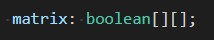
\includegraphics[scale=0.8]{matrix_matrix_def}
                    \caption{Declararea matricii}
                \end{figure}

            \paragraph{}
                \textbf{Starea celulelor} este modificata de către clasa din care fac parte, astfel celula in sine are doar funcționalitatea de a-si retine propria stare.

            \paragraph{}
                \textbf{Regulile de evoluție} sunt oferite de către un obiect ce deține o listă de reguli.
                Acest obiect este inițializat folosind setul de reguli de baza. Obiectul conține o listă de cerințe.
                Fiecare cerința are la rândul ei o lista de intervale si un set de condiții logice.
                Aceste condiții sunt folosite pentru a determina daca un anumit scenariu se aplica.
                In cazul in care scenariul est confirmat ca fiind potrivit pentru starea actuala se folosește un alt set intern de condiții ce stabilesc starea următoare a celulei.
            
            \paragraph{}
                \textbf{Evolutia celuleror} este realizata de o metoda a clasei.
                Aceasta funcție analizează datele ce sunt prezente in generația actuala si folosește instrucțiunile oferite de către serul de reguli pentru a genera următoare generație.

            \paragraph{}
                \textbf{Dimensiunea simulării} este predefinita dar se poate mari sau micșora folosind interfața grafica.
                Modificarea simulării nu duce la pierderea stării, excepție de la aceasta regula o face micșorarea simulării astfel încât celulele depășesc limita acesteia.
                Atât mărirea cat si micșorarea se face începând in coltul cel mai îndepărtat fata de origine.

        \subsection{Implementarea interfeței grafice}
            \paragraph{}
                Acest sistem pune accent pe implementarea modelului multi-agent, astfel interfața comanda si afișează starea simulării.
                Astfel arhitectura necesara implementării interfeței nu afectează sistemul simulat.

            \paragraph{}
                \textbf{Compatibilitatea dintre sistem si interfața grafica} se face folosind interfețele.
                Sistemul multi-agent implementează o interfața ce permite interfeței grafice sa acceseze resursele necesare acesteia.
                \begin{figure}[h]
                    \centering
                    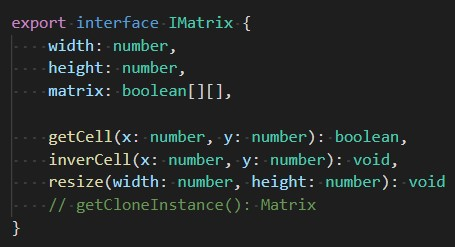
\includegraphics[scale=0.8]{IMatrix_interface}
                    \caption{Interfața implementata de matrice}
                \end{figure}

                De asemenea interfața grafica are mai multe implementări ce implementează si ele la rândul lor o interfață.



            \paragraph{}
                \textbf{Interfața grafica} este implementata folosind doua sisteme diferita: componente web native si implementarea grafica folosind o librărie grafica specializata.
                Acestea doua implementări sunt abstractizate si pot fi interschimbate  in timp real de către utilizator.
                \begin{figure}[h]
                    \centering
                    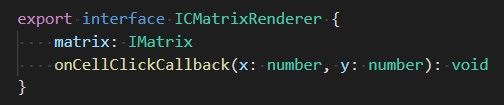
\includegraphics[scale=0.8]{ICMatricRenderer_interface}
                    \caption{Interfața implementata de sistemele de randare}
                \end{figure}

    \section{Funcționarea programului pentru experimentare}

        

    \section{Cazuri experimentale}

    \section{Probleme întâlnite}

        \paragraph{} Simularile multi-agent prezinta multe obstacole si probleme. Principalele dificultati in cadrul acestui proiect sunt:
        \begin{itemize}
            \item Implementarea sistemului ce retine si modifica starea agenților.
            Acest sistem poate fi implementat folosind diferite structuri de date, cum ar fi: matricile sau listele.
            Principalul avantaj al matricii este accesul direct al al oricarui agent dar si al vecinilor acestuia, un mare desavantaj este fapul ca odata cu cresterea dimensiunii sumularii creste si marimea matricii.
            Simularea folosind liste permite o scalare mai usoara si o separare dintre numarul total de agenti posibil si marimea mediului de simulare.
            Cel mai mare dezavantaj consta in faptul ca anumite operatii sunt mult mai greu de implementat si necesita mult mai multi pasi de executie.
            In cazu acesui proiect matricea a fost solosita ca si mijloc de stocare al datelor.

            \item Implementarea si unei interfete grafice ce permite interactiunea directa cu simularea. Interfata grafica si simularea necesita arhitecturi total diferite. Deci simularea sistemului este punctul de referinta, interfata grafica afiseaza si modifica datele la cererea utilizatorului.
        \end{itemize}

    \section{Modificările si îmbunătățirile necesare}

    \section{Referințe}

        \begin{itemize}
            \item \href{https://en.wikipedia.org/wiki/Conway%27s_Game_of_Life}{wiki | Conway's Game of Life}
        \end{itemize}


\end{document} 